% !TEX root =  ../pers_schedules.tex 

\section{Simulation study}
\label{sec: simulation_study}
The application of personalized schedules for patients from PRIAS demonstrated that the schedules adapt according to the historical data of each patient. However we could not perform a full scale comparison between personalized and PRIAS schedules, because the true time of GR was not known for any of the PRIAS patients. To this end, we have performed a simulation study comparing personalized schedules based on expected time of GR, median time of GR and dynamic risk of GR, with a hybrid approach between median time of GR and dynamic risk of GR, PRIAS schedule and annual schedule. We employ these schedules for simulated patients enrolled in a hypothetical AS program, with the same entrance criteria as PRIAS.

\subsection{Simulation setup}
\label{subsec : simulation_setup}
First we assume a population of patients enrolled in AS, whose PSA and hazard of GR follows a joint model of the form postulated in Section \ref{subsec : jm_fit_prias}, with parameters equal to the posterior mean of parameters (Web Appendix C of the supplementary material) estimated from the joint model fitted to PRIAS dataset. To check the efficacy of personalized schedules in scenarios with a mixture of patients, with early as well as late failure times, we assume that the patient population belongs to three equal sized subgroups $G_1, G_2, G_3$. The failure times in each subpopulation are controlled by different Weibull distributed baseline hazards for each. The corresponding shape and scale parameters $(k, \lambda$) are: $(1.5, 4)$, $(3, 5)$ and $(4.5, 6)$ for subgroups $G_1, G_2$ and $G_3$, respectively. The effect of these parameters is that the variance in time of GR is highest for $G_1$ and lowest for $G_3$, while the mean GR time is lowest in $G_1$ and highest in $G_3$.

From this population we have sampled 500 datasets with 1000 patients each. Patients are randomly assigned to a subgroup. Further, each dataset is split into a training (750 patients) and a test (250 patients) part. The $k$-th simulated training dataset $\mathcal{D}^k$ is given by $\mathcal{D}^k = \{l_{ki}, r_{ki}, \boldsymbol{y}_{ki}; i = 1, \ldots, 750\}$, where $\boldsymbol{y}_{ki}$ denote the PSA measurements for the $i$-th patient in $\mathcal{D}^k$. The frequency of PSA measurements is same as that in PRIAS. Other than simulating a true GR time $T^*_{ki}$, we also generate a random and non-informative censoring time $C_{ki}$. When $T_{ki} < C^*_{ki}$, then $l_{ki} = r_{ki} = T^*_{ki}$, otherwise $l_{ki} = C_{ki}$ and $r_{ki} = \infty$. For the test patients, censoring time is not generated.

\subsection{Estimation}
We fit a joint model of the specification given in (\ref{eq : long_model_prias}) and (\ref{eq : hazard_prias}) to each of the $\mathcal{D}^k, k=1,
\ldots, 500$, and obtain a MCMC sample from the posterior distribution $p(\boldsymbol{\theta} \mid \mathcal{D}^k)$. We next obtain $g(T^*_{kj})$ for the $j$-th test patient and conduct hypothetical biopsies iteratively in accordance with the algorithm in Figure \ref{fig : sched_algorithm}. 	[TALK ABOUT DIFFERENT METHODS YOU COMPARE, AND HOW YOU COMPARE THEM....AND STILL IN ESTIMATION???] 

To compare schedules we require estimates of the various measures of efficacy of schedules (Section \ref{sec : choosing_schedule}). To this end, we compute pooled estimates of each of the $E[N^{bS}]$, $\mbox{var}[N^{bS}]$, $E[O^S]$ and $\mbox{var}[O^S]$, as below:
\begin{align*}
\widehat{E[O^S]} &= \frac{\sum_{k=1}^{500} n_k \widehat{E[O^S_k]}}{\sum_{k=1}^{500} n_k}, \\
\widehat{\mbox{var}[O^S]} &= \frac{\sum_{k=1}^{500} (n_k - 1) \widehat{\mbox{var}[O^S_k]}}{\sum_{k=1}^{500} (n_k-1)}, 
\end{align*}
where $n_k$ denotes the number of test patients, $\widehat{E[O^S_k]} = {\sum_{j=1}^{n_k}O^S_{kj}}/{n_k}$ is the estimated mean and $\widehat{\mbox{var}[O^S_k]} = {\sum_{j=1}^{n_k}\big\{O^S_{kj} - \widehat{E[O^S_k]}\big\}^2}/{n_k-1}$ is the estimated variance of the offset for the $k$-th simulation. The estimates for number of biopsies $N^{bS}$ are obtained similarly.

\subsection{Results}
The pooled estimates of the various measures of efficacy are summarized in Table \ref{table : sim_study_pooled_estimates}. In addition mean offset is plotted against mean number of biopsies in Figure \ref{fig : meanNbVsOffset}. From the figure it is evident that there is an inverse relationship between $E[N^{bS}]$ and $E[O^S]$. For example, the annual schedule conducts 5.2 biopsies on average, which is the highest among all schedules, however it has the least average offset of 6 months as well. On the other hand the schedule based on expected time of GR conducts only 1.9 biopsies on average, the least among all schedules, but it also has the highest average offset of 15 months. The schedule based on median time of GR performs similar to that based on expected time of GR. Since the annual schedule attempts to contain the offset within an year it has the least $\mbox{var}[O^S]$. However to achieve so, it conducts a wide range of number of biopsies from patient to patient, i.e. highest $\mbox{var}[N^{bS}]$. Schedules based on expected and median time of GR perform the opposite of annual schedule in terms of variance of $N^{bS}$ and $O^S$.

\begin{figure}
\centerline{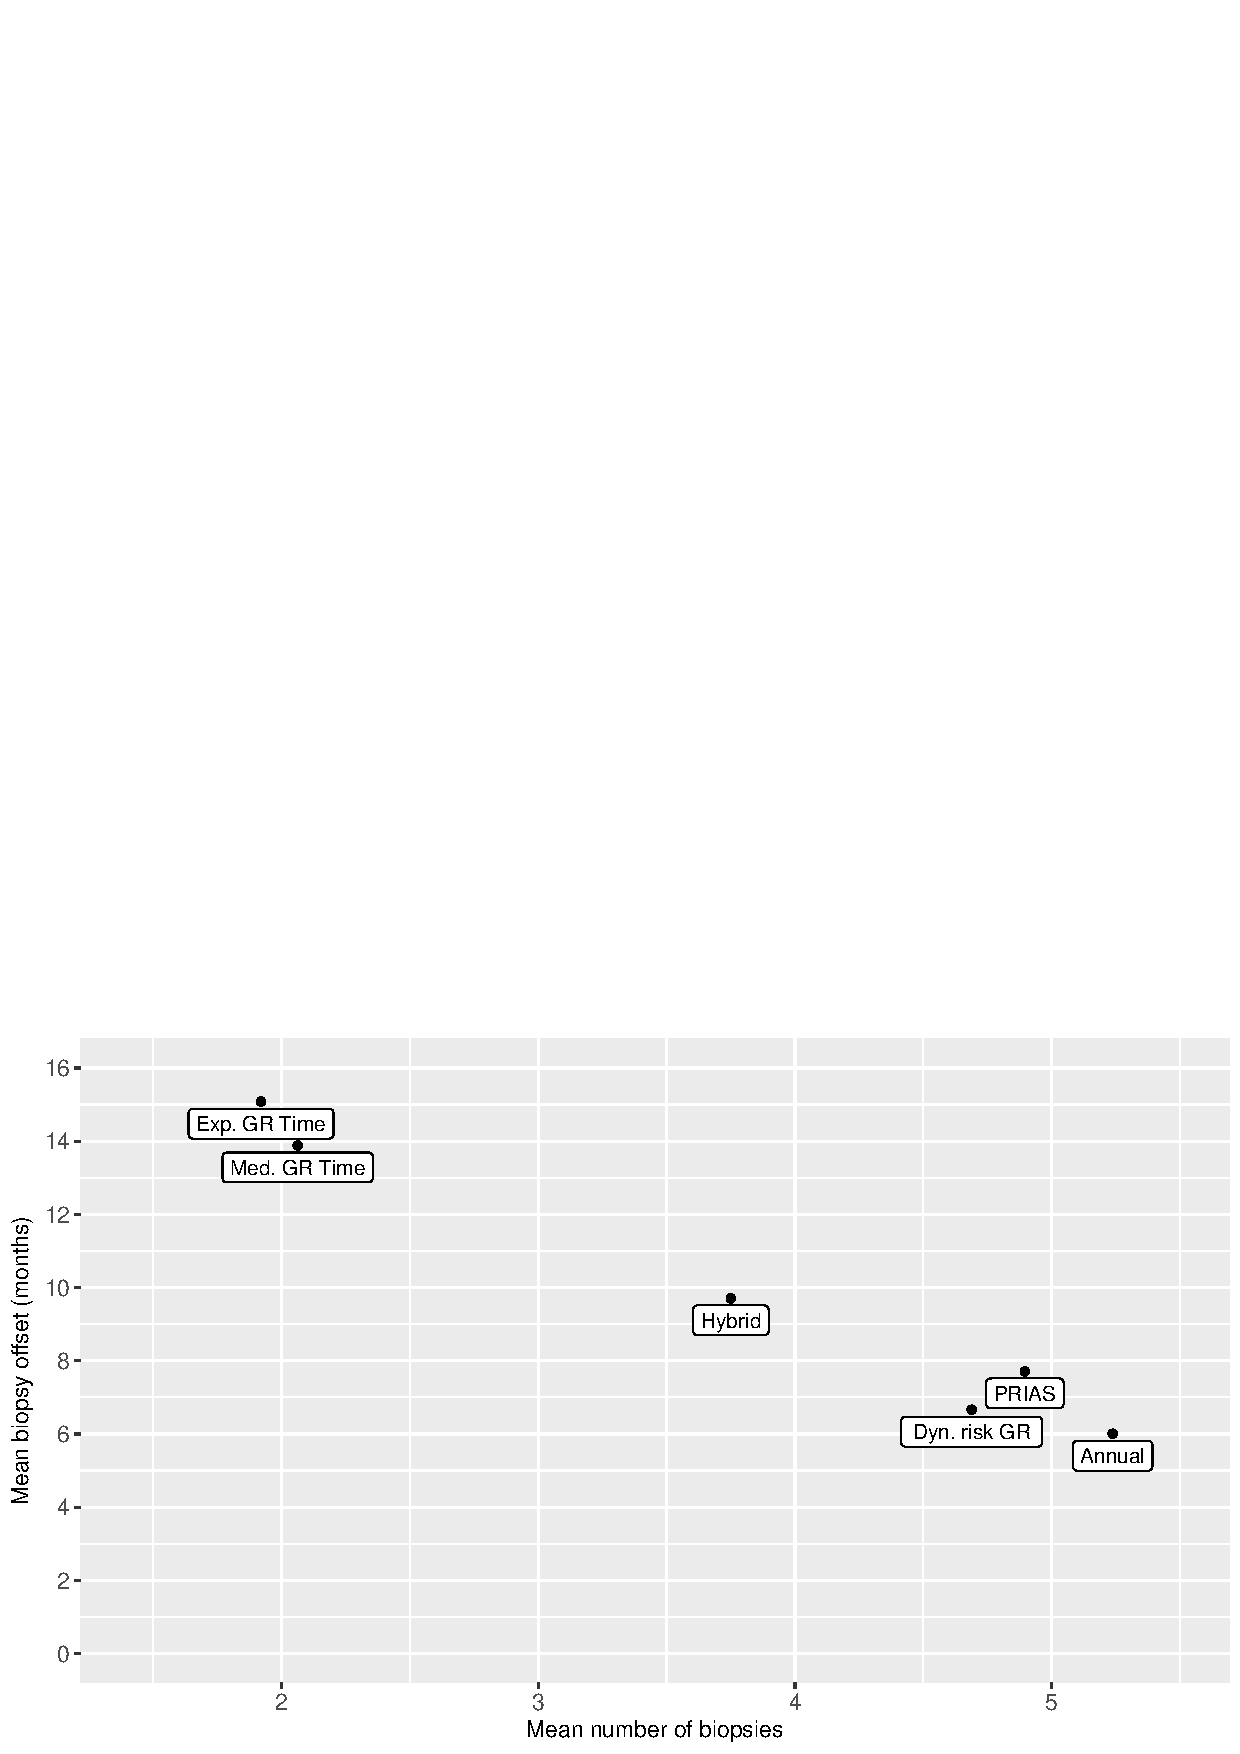
\includegraphics[width=\columnwidth]{images/sim_study/meanNbVsOffset_all.png}}
\caption{Estimated mean number of biopsies and mean offset (months) for the 6 schedules, using all subgroups. Method names are abbreviated for better readability.}
\label{fig : meanNbVsOffset}
\end{figure}

\begin{table}
\caption{Estimated mean and standard deviation of the number of biopsies and offset (months). Method names are abbreviated for consistency with Figure \ref{fig : meanNbVsOffset}.}
\label{table : sim_study_pooled_estimates}
\begin{tabular}{lrrrr}
\Hline
\multicolumn{5}{c}{a) All subgroups: 101823 patients}\\
\hline
Schedule          & $E[N^{bS}]$ & $E[O^{S}]$ & ${\mbox{SD}[N^{bS}]}$ & ${\mbox{SD}[O^S]}$ \\
\hline
Annual         & 5.24            & 6.01                & 2.53          & 3.45              \\
PRIAS          & 4.86            & 8.49                & 2.35          & 8.69\\
Exp. GR time & 1.92            & 15.06               & 1.19          & 12.11             \\
Med. GR time & 2.07            & 13.87               & 1.42          & 11.80              \\
Dyn. risk GR       & 4.69            & 6.66                & 2.20           & 4.37              \\
Mixed       & 3.75            & 9.69                & 1.71          & 7.02              \\
\hline
\multicolumn{5}{c}{b) Subgroup $G_1$: 33680 patients}\\
\hline
Schedule        & $E[N^{bS}]$ & $E[O^{S}]$ & ${\mbox{SD}[N^{bS}]}$ & ${\mbox{SD}[O^S]}$ \\
\hline
Annual         & 4.33            & 6.02                & 3.14          & 3.44              \\
PRIAS          & 4.05            & 7.98                & 2.87          & 8.08     \\
Exp. GR time & 1.72            & 21.65               & 1.47          & 14.77             \\
Med. GR time & 1.85            & 20.67               & 1.77          & 14.64             \\
Dyn. risk GR       & 3.85            & 6.76                & 2.69          & 4.45              \\
Mixed       & 3.24            & 10.24               & 2.17          & 7.73              \\
\hline      
\multicolumn{5}{c}{c) Subgroup $G_2$: 33907 patients}\\
\hline
Schedule        & $E[N^{bS}]$ & $E[O^{S}]$ & ${\mbox{SD}[N^{bS}]}$ & ${\mbox{SD}[O^S]}$ \\
\hline
Annual         & 5.18            & 5.99                & 2.13          & 3.48              \\
PRIAS          & 4.82            & 8.57                & 1.99          & 8.65        \\
Exp. GR time & 1.78            & 13.53               & 0.98          & 9.82              \\
Med. GR time & 1.90             & 12.31               & 1.16          & 9.43              \\
Dyn. risk GR       & 4.63            & 6.66                & 1.82          & 4.34              \\
Mixed       & 3.68            & 10.30                & 1.38          & 7.17              \\
\hline      
\multicolumn{5}{c}{d) Subgroup $G_3$: 34236 patients}\\
\hline
Schedule        & $E[N^{bS}]$ & $E[O^{S}]$ & ${\mbox{SD}[N^{bS}]}$ & ${\mbox{SD}[O^S]}$ \\
\hline
Annual         & 6.2             & 6.01                & 1.77          & 3.46              \\
PRIAS          & 5.70             & 8.92                & 1.73          & 9.27        \\
Exp. GR time & 2.27            & 10.11               & 0.99          & 7.53              \\
Med. GR time & 2.45            & 8.71                & 1.15          & 6.36              \\
Dyn. risk GR       & 5.57            & 6.58                & 1.56          & 4.32              \\
Mixed       & 4.31            & 8.54                & 1.27          & 5.91              \\
\hline     
\end{tabular}
\end{table}

The PRIAS schedule conducts only 0.4 biopsies less than annual schedule, but with a higher variance of offset, it does not guarantee early detection for everyone. If we compare the PRIAS schedule with dynamic risk of GR based schedule, we can see that the latter performs better than PRIAS schedule in all aspects. The hybrid approach combines the benefits of methods with low $E[N^{bS}]$ and $\mbox{var}[N^{bS}]$, and methods with low $E[O^{S}]$ and $\mbox{var}[O^S]$. It conducts 1.5 less biopsies than annual schedule on average and with $E[O^{S}]$ at 9.7 months it detects GR within an year since its occurrence. The variance in number of biopsies and offset are not only not high but also lesser than PRIAS schedule.

We next discuss the performance of these schedules for each of the 3 subgroups $G_1, G_2$ and $G_3$. We observe that annual schedule remains the most consistent across subgroups in terms of the offset, but it varies the most in terms of number of biopsies, conducting 2 extra biopsies in subgroup $G_3$ (highest mean, low variance of GR time) than in $G_1$ (low mean, high variance of GR time). The performance of schedule based on expected time of GR is the most consistent in terms of number of biopsies but most inconsistent in terms of offset. It performs the best in subgroup $G_3$. For the dynamic risk of GR based schedule and the hybrid approach the dynamics are similar to that of the annual schedule. Unlike the latter two schedules, the PRIAS schedule not only conducts more biopsies in $G_3$ than $G_1$ but also has a higher offset for $G_3$ than $G_1$.

The choice of the optimal schedule using (\ref{eq : loss_func_sim_study_generic}) depends on the chosen measures of efficacy. For example, schedule based on dynamic risk of GR is the most optimal if on average the least number of biopsies are to be conducted, while simultaneously making sure that at least 90\% of the patients have an average offset less than an year. Schedule based on expected time of GR is most optimal if on average the least number of biopsies are to be conducted, while simultaneously making sure that at least 80\% of the patients have an average offset less than 2 years. For at least 90\% of the patients it detects GR within 3 years with 2 biopsies on average. We however recommend the hybrid approach, since it conducts only 3.8 biopsies on average while guaranteeing an offset of 24 months for 95\% of the patients and 36 months for 99.9\% of the patients. Besides if further cutoffs are required on variance of number of biopsies or offset they are not too high either for the hybrid approach.